% 5章
\chapter{数値実験}

研究で新たに実装した歩行者工一ジェントおよび介護シミュレーションの定量的な評価性能を検証するために,シミュレーション実験を行った.
この章では,実験で用いた環境設定と,実験結果をどのような評価指標で判断したか,またその結果と考察についてまとめている.

\section{実験条件}

今回の実験では介護環境として,図\ref{environment}に示すように,15m四方の二次元平面と,排泄場所としてのトイレをその上部に設置した.

\begin{figure}[htb]
\begin{center}
 
\includegraphics[scale=0.5]{figures/environment.png}
 \caption[実験環境]{実験環境 \label{environment}}
\end{center}
\end{figure}

この環境の中で,介護者と被介護者の可視化をおこなっていく.今回の実験では,介護における技術を導入した際に,それが介護環境にどのようなインパクトをあたえるのかについて検証を行うことが目的なので,介護者の数は1人,被介護者の数は16人と設定し,比較的大きい施設を対象とした.第4章で述べた健常者,頻尿の被介護者,認知症の被介護者の3種類のエージェントが,介護施設内の自由時間である2時間の間にいかなる回数にわたって排泄介助を行うことが必要か,またその介助は本当に必要であったのかということを確かめる実験をおこなう.3種類の被介護エージェントを\ref{experiment}のように組み合わせた6パターンにおいて,相互作用を確認し,それを本章で示す評価指標で評価する.

\begin{figure}[htb]
\begin{center}
 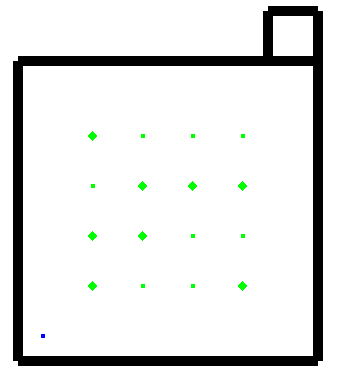
\includegraphics[scale=0.5]{figures/health_urinate.png}
 \caption[健常者と認知症の場合の可視化]{健常者と認知症の場合の可視化 \label{health_urinate}}
\end{center}
\end{figure}

\begin{figure}[htb]
\begin{center}
 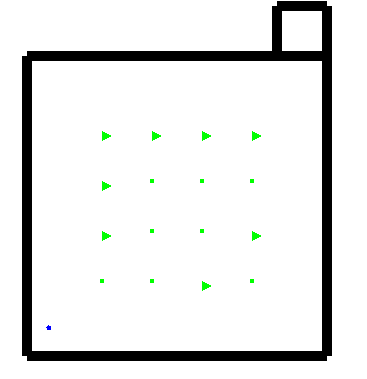
\includegraphics[scale=0.5]{figures/health_frequently_urinate_v1.png}
 \caption[健常者と頻尿の場合の可視化]{健常者と頻尿の場合の可視化 \label{health_frequently_urinate_v1}}
\end{center}
\end{figure}

\begin{figure}[htb]
\begin{center}
 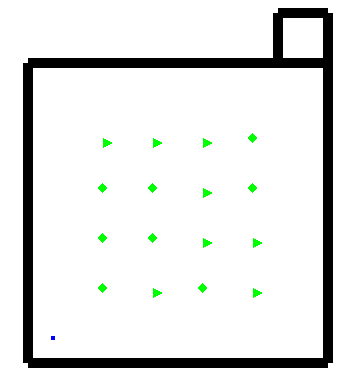
\includegraphics[scale=0.5]{figures/dementia_urinate_v1.png}
 \caption[認知症と頻尿の場合の可視化]{認知症と頻尿の場合の可視化 \label{dementia_urinate_v1}}
\end{center}
\end{figure}

表\ref{experiment}に示したように,Case1は、健常の被介護者(技術の補助を受けた被介護者)が100%の状態,Case2は頻尿の被介護者が100%の状態,Case3は認知症の被介護者が100%の状態,Case4は、健常の被介護者(技術の補助を受けた被介護者)と頻尿の被介護者が50%ずつの状態,Case5は健常の被介護者(技術の補助を受けた被介護者)と認知症の被介護者が50%ずつの状態,Case6は頻尿の被介護者と認知症の被介護者が50%ずつの状態である.

\section{介護挙動の基本的な検証}

本シミュレータが現実を反映できているのかについて,簡単な検証を行った.介護アラートを出す条件を,健常者の場合は100ml以上になった時点,頻尿の場合は75ml以上になった時点,認知症の場合は150ml以上で介護アラートを発する設定にし,2時間シミュレータを回した.その結果,健常者の場合は,2時間に1回トイレに行くという結果を得ることができた.これは実際のデータと比較しても整合性のある値となった.この結果を表\ref{number_of_urination}に示す.なお,実験では16人の被介護者が存在するので実際は数値を16で割った数字が一人当たりの回数となっている.

\begin{table}[htb]
  \caption[被介護者ごとの排尿回数]{被介護者ごとの排尿回数}
  \label{number_of_urination}
  \centering
  \begin{tabular}{r|c|c|c}
     & 健常者 & 頻尿 & 認知症 \\ \hline
    一回目 & 15 & 21 & 6 \\
    二回目 & 15 & 22 & 5 \\
    三回目 & 16 & 26 & 5 \\
    \end{tabular}
\end{table}

\section{評価指標}

本研究の目的は,疾患のある被介護者,すなわち現状介護者の負担増の原因となっており,被介護者自身も自らの排泄が負担となっているようなケースにおいて,技術の導入を行うことでどれだけの効果が得られるのかを可視化するというものである.そこで,評価指標としては,排泄に行くべきである尿量の状態,あるいは自身が排泄に行きたいと感じている状態から実際に排泄を行うまでの時間を計測し,それを総我慢時間とし,本研究の評価指標とする.

\section{結果および考察}

図\ref{result_v1}に,介護者・被介護者の割合をCase1からCase6までそれぞれ変化させた場合のシミュレーション結果(10回の試行の平均値)を示す.また,表\ref{relative_error}に,Case1に対する相対誤差を示した.次に表\ref{number_of_care}に,Caseごとの介護回数とCase1に対する相対誤差を示した.

\begin{figure}[htb]
\begin{center}
 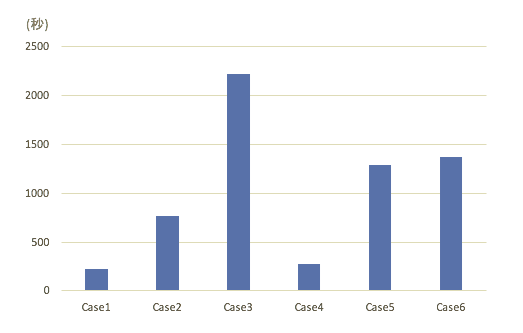
\includegraphics[scale=0.5]{figures/result_1.png}
 \caption[実験結果]{実験結果 \label{result_v1}}
\end{center}
\end{figure}

\begin{table}[htb]
  \caption[Case1に対する相対誤差]{Case1に対する相対誤差}
  \label{relative_error}
  \centering
  \begin{tabular}{r|c|c|c|c|c}
     & Case2 & Case3 & Case4 & Case5 & Case6 \\ \hline
    相対誤差 & 2.47 & 9.05 & 0.26 & 4.84 & 5.19 \\
    \end{tabular}
\end{table}


\begin{table}[htb]
  \caption[Caseごとの介護回数]{Caseごとの介護回数}
  \label{number_of_care}
  \centering
  \begin{tabular}{r|c|c|c|c|c|c}
     & case1 & Case2 & Case3 & Case4 & Case5 & Case6 \\ \hline
    介護回数 & 15-16 & 21-26 & 5-6 & 19-21 & 9-10 & 16-17 \\
    相対誤差 & & 0.50 & -0.65 & 0.31 & -0.37 & 0.07 \\
    \end{tabular}
\end{table}

Case3の総我慢時間が,もっとも高いものとなっているが,これは被介護者が本来なら排泄に向かうべき尿量であるのにも関わらず,無意識のうちに我慢をしてしまい,介護者にアラートを出した時点ですでにかなりの時間を待ち時間として計測してしまっていることが原因であることが考えられる.Case5では,数値上は相対誤差がかなり少ないように見えるが,実際は健常者と認知症の被介護者の間の待ち時間の差が大きく,健常者の割合が減ったことで,健常者がアラートを出した際にすぐ介護してもらえたということがあげられる.実際の現場では,被介護者の要介護によって,どの介護者がつくべきかということが事前情報として与えられているため,このような複雑な状況にも対応していけるような環境をつくっているという示唆を得ることができる.今後の検討課題として,そういった事前情報の有無によって,どの介護者と被介護者をマッチングさせるのかということが挙げられる.Case2については,過剰介護が問題であると考えられる.健常者の場合と比べ,50%以上も介護士の労働力に悪影響を与えているといえる.
